% ============================================================
% FEDMED-X CAPSTONE REPORT — MAIN DRIVER FILE
% Bangladesh University of Business and Technology (BUBT)
% Compiled with: pdflatex -> biber -> pdflatex -> pdflatex
% ============================================================

\documentclass[12pt,a4paper,oneside]{report}

% ──────────────────────────────────────────────────────────
% PACKAGES (same as preamble.tex, inlined for flat compile)
% ──────────────────────────────────────────────────────────
\usepackage[a4paper,top=1in,bottom=1in,left=1.25in,right=1in]{geometry}
\usepackage[T1]{fontenc}
\usepackage[utf8]{inputenc}
\usepackage{lmodern}
\usepackage{microtype}

% Spacing
\usepackage{setspace}
\onehalfspacing
\setlength{\parskip}{4pt plus 1pt minus 1pt}

% Math + graphics
\usepackage{amsmath,amssymb,amsfonts}
\usepackage{graphicx}
\usepackage{xcolor}
\usepackage{float}
\usepackage{placeins}

% TikZ
\usepackage{tikz}
\usetikzlibrary{shapes.geometric,arrows.meta,positioning,fit,calc,backgrounds,shadows}

% Tables
\usepackage{booktabs,tabularx,longtable,multirow,array,makecell}
\usepackage{ragged2e}

% Lists
\usepackage{enumitem}
\setlist{itemsep=2pt,topsep=3pt}

% Captions
\usepackage[labelfont=bf,font=small,justification=centering]{caption}

% Headers/footers
\usepackage{fancyhdr}
\pagestyle{fancy}
\fancyhf{}
\renewcommand{\headrulewidth}{0.4pt}
\fancyhead[L]{\small\itshape FEDMED-X}
\fancyhead[R]{\small\itshape BUBT Capstone 2026}
\fancyfoot[C]{\thepage}

% ──────────────────────────────────────────────────────────
% TOC / LOF / LOT FORMATTING  (matching report theme)
% ──────────────────────────────────────────────────────────
\usepackage{tocloft}

% --- Table of Contents ---
\renewcommand{\cfttoctitlefont}{\normalfont\Large\bfseries}
\renewcommand{\cftaftertoctitle}{\par\nobreak\vskip 6pt%
  \hrule height 0.4pt \vskip 10pt}
\setlength{\cftbeforetoctitleskip}{0pt}
\setlength{\cftaftertoctitleskip}{6pt}

% --- List of Figures ---
\renewcommand{\cftloftitlefont}{\normalfont\Large\bfseries}
\renewcommand{\cftafterloftitle}{\par\nobreak\vskip 6pt%
  \hrule height 0.4pt \vskip 10pt}
\setlength{\cftbeforeloftitleskip}{0pt}
\setlength{\cftafterloftitleskip}{6pt}

% --- List of Tables ---
\renewcommand{\cftlottitlefont}{\normalfont\Large\bfseries}
\renewcommand{\cftafterlottitle}{\par\nobreak\vskip 6pt%
  \hrule height 0.4pt \vskip 10pt}
\setlength{\cftbeforelottitleskip}{0pt}
\setlength{\cftafterlottitleskip}{6pt}

% Dot leaders for all list levels
\renewcommand{\cftchapdotsep}{\cftdotsep}
\renewcommand{\cftsecdotsep}{\cftdotsep}

% Chapter title formatting (matches BUBT template)
\usepackage{titlesec}
\titleformat{\chapter}[display]
  {\normalfont\Large\bfseries\centering}
  {Chapter \thechapter}{12pt}{\Large}
\titlespacing*{\chapter}{0pt}{-10pt}{20pt}

% Hyperlinks
\usepackage[hidelinks]{hyperref}
\hypersetup{
  colorlinks=true,
  linkcolor=black,
  citecolor=black,
  urlcolor=blue,
  pdftitle={FEDMED-X Capstone Report},
  pdfauthor={Mohammad Zunayed and Team}
}

% Bibliography (IEEE style)
\usepackage[backend=biber,style=ieee,sorting=none,maxbibnames=99]{biblatex}
\addbibresource{references.bib}

% Custom Summary command (chapter-end)
\newcommand{\chaptersummary}[1]{%
  \vspace{6pt}\noindent\textbf{Summary}\\[2pt]#1\par\vspace{6pt}
}

% ──────────────────────────────────────────────────────────
\begin{document}

% ── COVER PAGE ──────────────────────────────────────────
\pagestyle{empty}
\begin{titlepage}
\centering
\vspace*{0.2in}

\rule{\textwidth}{1.2pt}\\[10pt]
{\large\bfseries FEDMED-X: Communication-Efficient Privacy-Preserving\\
Federated Learning with Real Edge Hardware Deployment for\\
Medical Image Classification\par}
\vspace{10pt}
\rule{\textwidth}{1.2pt}\\[25pt]

{\normalsize By\par}
\vspace{10pt}

\begin{tabular}{ll}
Mohammad Zunayed   \hspace{1.2cm} & ID: 20234103328 \\[4pt]
Md. Najmush Shakib \hspace{1.2cm} & ID: 20234103357 \\[4pt]
Munim Halder       \hspace{1.2cm} & ID: 20234103351 \\[4pt]
Md. Nur Alam       \hspace{1.2cm} & ID: 20234103153 \\[4pt]
Omar Faruk Jihad   \hspace{1.2cm} & ID: 20234103145 \\
\end{tabular}

\vspace{20pt}
{\bfseries Supervisor}\\[6pt]
Md. Saddam Hossain\\
Assistant Professor, CSE, BUBT

\vspace{20pt}
Submitted in partial fulfillment of the requirements of the degree of\\
{\bfseries Bachelor of Science in}\\
{\bfseries Computer Science and Engineering}

\vspace{15pt}
\IfFileExists{BUBT-Logo.png}
  {
\includegraphics[width=2.4cm]{BUBT-Logo.png}}
  {\fbox{\parbox[c][2.2cm][c]{2.2cm}{\centering\small BUBT\\LOGO}}}

\vspace{10pt}
Department of Computer Science and Engineering\\
Bangladesh University of Business and Technology

\vfill
7 September 2026
\end{titlepage}   % uncomment if cover_page.tex exists
\clearpage

% ── FRONT MATTER (roman numerals) ───────────────────────
\pagenumbering{roman}
\setcounter{page}{2}
\pagestyle{plain}

\chapter*{Declaration}
\addcontentsline{toc}{chapter}{Declaration}

We do hereby declare that the research works presented in this thesis entitled,
\textit{``FEDMED-X: Communication-Efficient Privacy-Preserving Federated
Learning with Real Edge Hardware Deployment for Medical Image
Classification''} are the results of our own works. We further declare that the
thesis/report has been compiled and written by us, and no part of this
thesis/report has been submitted elsewhere for the requirements of any degree,
award, diploma, or any other purposes except for publications. The materials
that are obtained from other sources are duly acknowledged in this thesis.

\vspace{25pt}
\noindent\underline{\textbf{Signature of Authors}}

\vspace{20pt}
\noindent
\begin{tabularx}{\textwidth}{@{}XX@{}}
\rule{5cm}{0.4pt} & \rule{5cm}{0.4pt} \\
\textbf{Mohammad Zunayed}       & \textbf{Md. Najmush Shakib} \\
ID: 20234103328                 & ID: 20234103357             \\[24pt]
\rule{5cm}{0.4pt} & \rule{5cm}{0.4pt} \\
\textbf{Munim Halder}           & \textbf{Md. Nur Alam}        \\
ID: 20234103351                 & ID: 20234103153              \\[24pt]
\rule{5cm}{0.4pt} &                                            \\
\textbf{Omar Faruk Jihad}       &                              \\
ID: 20234103145                 &                              \\
\end{tabularx}
\chapter*{Approval}
\addcontentsline{toc}{chapter}{Approval}

It is hereby certified that the research work presented in this thesis entitled,
\textit{``FEDMED-X: Communication-Efficient Privacy-Preserving Federated
Learning with Real Edge Hardware Deployment for Medical Image
Classification,''} is the result of the original work carried out by Mohammad
Zunayed, Md. Najmush Shakib, Munim Halder, Md. Nur Alam, and Omar Faruk
Jihad. Furthermore, it is certified that this thesis/report satisfies the
requirements and standards for the degree of Bachelor of Science in Computer
Science and Engineering.

\vspace{18pt}

\noindent
\begin{tabularx}{\textwidth}{@{}p{7.5cm}X@{}}
\rule{6cm}{0.4pt} & \\
\textbf{Md. Saddam Hossain}          & \textbf{Supervisor} \\
Assistant Professor, CSE             & Capstone Defense Board \\
BUBT, Dhaka                          &  \\[22pt]

\rule{6cm}{0.4pt} & \\
\textbf{Dr. Md. Rajibul Islam}       & \textbf{Member (Internal)} \\
Associate Professor, Data Science    & Capstone Defense Board \\
BUBT, Dhaka                          & \\[22pt]

\rule{6cm}{0.4pt} & \\
\textbf{Prof. Dr. Md. Ahsan Habib}   & \textbf{Convener} \\
Chairman, CSE                        & Capstone Defense Board \\
BUBT, Dhaka                          & \\
\end{tabularx}

\vspace{22pt}
\begin{center}
\textbf{Department of Computer Science and Engineering, BUBT, Dhaka.}
\end{center}
\chapter*{Dedication}
\addcontentsline{toc}{chapter}{Dedication}
\vspace{25pt}
\begin{center}
\itshape
``We dedicate this research to our loving parents,\\
whose unwavering love, encouragement, sacrifices,\\
and constant support have been the foundation of our\\
academic journey.

\vspace{14pt}
This work is also dedicated to our respected teachers,\\
particularly our supervisor Md. Saddam Hossain,\\
whose academic vision and mentorship shaped every aspect\\
of this research.

\vspace{14pt}
Finally, we dedicate this work to the underserved patients\\
and rural healthcare workers of Bangladesh, whose need for\\
affordable, private, and reliable diagnostic tools\\
motivated the design of FEDMED-X.''
\end{center}
\chapter*{Acknowledgement}
\addcontentsline{toc}{chapter}{Acknowledgement}

We would like to express our heartfelt gratitude to the Almighty Allah, who
offered our families and us kind care throughout this journey. We are deeply
thankful to the Bangladesh University of Business and Technology (BUBT) for
providing us with an excellent research environment and world-class computing
facilities to pursue our capstone project.

We express our sincerest gratitude to our respected supervisor,
\textbf{Md.~Saddam Hossain}, Assistant Professor, Department of CSE, BUBT.
This research would not have been possible without his patient guidance, sharp
technical insight, and consistent academic support. He identified the research
gap in privacy-preserving federated learning for edge medical devices, guided
us through the complex integration of FedProx, Differential Privacy, and
gradient compression, and shared many essential research resources. He was
disciplined and responsible, always finding time to discuss our progress.

We are also thankful to our course teacher, \textbf{Dr.~Md.~Rajibul Islam},
Associate Professor and Chairman of the Department of Data Science and
Engineering, BUBT, for providing valuable direction and constructive academic
feedback throughout the semester. Special appreciation goes to
\textbf{Prof.~Dr.~Md.~Ahsan Habib}, Chairman of the CSE Department, and to
all our respected faculty members for their consistent inspiration.

We would also like to acknowledge our five-member team for their coordinated
technical effort, patience, and mutual encouragement throughout the eight-month
development cycle. Finally, we are grateful to our families, well-wishers, and
BUBT for granting us this opportunity to contribute to trustworthy artificial
intelligence in healthcare.
\chapter*{Abstract}
\addcontentsline{toc}{chapter}{Abstract}

Federated Learning (FL) enables collaborative medical image diagnosis without
sharing raw patient data, supporting privacy regulations such as HIPAA and
GDPR. In practice, medical FL faces non-IID data drift, communication
bottlenecks, and gradient-leakage risks. Existing studies often address these
issues separately and rarely evaluate full pipelines under edge constraints.
This report presents FEDMED-X, a communication-efficient and
privacy-preserving federated learning system for medical image classification.
The framework integrates FedProx ($\mu = 0.01$), DP-SGD ($\epsilon = 1.0$,
$\delta = 1 \times 10^{-5}$), TopK 50\% + INT8 compression, and a lightweight
MedNet-CBAM model designed for edge deployment. On MedMNIST PneumoniaMNIST
with 5 Dirichlet non-IID clients ($\alpha = 0.5$), FedProx reached 85.58\%
accuracy. With privacy and compression together, FEDMED-X achieved 75.16\%
accuracy while reducing communication by 90\% under $\epsilon = 1.0$.
Edge-oriented evaluation targets NVIDIA Jetson Nano deployment with 0.20~ms per
image inference latency.

\vspace{6pt}
\noindent\textbf{Keywords:} Federated Learning; Differential Privacy; Edge
Computing; Medical Image Classification; FedProx; TopK; Jetson Nano.

% ──────────────────────────────────────────────────────────
% TABLE OF CONTENTS
% ──────────────────────────────────────────────────────────
\clearpage
\phantomsection
\addcontentsline{toc}{chapter}{Table of Contents}
\tableofcontents

% ──────────────────────────────────────────────────────────
% LIST OF FIGURES
% ──────────────────────────────────────────────────────────
\clearpage
\phantomsection
\addcontentsline{toc}{chapter}{List of Figures}
\listoffigures

% ──────────────────────────────────────────────────────────
% LIST OF TABLES
% ──────────────────────────────────────────────────────────
\clearpage
\phantomsection
\addcontentsline{toc}{chapter}{List of Tables}
\listoftables

% ── ABBREVIATIONS ────────────────────────────────────────
\clearpage
\chapter*{List of Abbreviations and Acronyms}
\addcontentsline{toc}{chapter}{List of Abbreviations and Acronyms}

\vspace{6pt}
\noindent
\begin{tabularx}{\textwidth}{@{}p{2.6cm}X@{}}
\textbf{AI}       & Artificial Intelligence \\
\textbf{BUBT}     & Bangladesh University of Business and Technology \\
\textbf{CBAM}     & Convolutional Block Attention Module \\
\textbf{CNN}      & Convolutional Neural Network \\
\textbf{DL}       & Deep Learning \\
\textbf{DP}       & Differential Privacy \\
\textbf{DP-SGD}   & Differentially Private Stochastic Gradient Descent \\
\textbf{FedAvg}   & Federated Averaging \\
\textbf{FedProx}  & Federated Proximal Optimization \\
\textbf{FL}       & Federated Learning \\
\textbf{FPS}      & Frames Per Second \\
\textbf{GDPR}     & General Data Protection Regulation \\
\textbf{GPU}      & Graphics Processing Unit \\
\textbf{HE}       & Homomorphic Encryption \\
\textbf{HIPAA}    & Health Insurance Portability and Accountability Act \\
\textbf{IID}      & Independent and Identically Distributed \\
\textbf{INT8}     & 8-bit Integer Quantization \\
\textbf{MedMNIST} & Medical MNIST Benchmark Dataset \\
\textbf{ML}       & Machine Learning \\
\textbf{RDP}      & R\'enyi Differential Privacy \\
\textbf{ReLU}     & Rectified Linear Unit \\
\textbf{SDLC}     & Software Development Life Cycle \\
\textbf{SOTA}     & State of the Art \\
\textbf{TopK}     & Top-K Gradient Sparsification \\
\end{tabularx}

% ── MAIN CHAPTERS (arabic page numbers) ─────────────────
\clearpage
\pagenumbering{arabic}
\setcounter{page}{1}
\pagestyle{fancy}

\chapter{Introduction}

Artificial Intelligence (AI) has transformed medical image analysis by enabling
automated detection of diseases from radiological scans such as chest X-rays.
Deep learning models can support clinicians in identifying pneumonia and
related abnormalities with high speed and consistency. However, building robust
medical AI systems requires large and diverse datasets collected across
multiple hospitals. In practice, hospitals cannot freely pool patient images
into a single central repository because of legal, ethical, and security
constraints. Privacy regulations such as the Health Insurance Portability and
Accountability Act (HIPAA) and the General Data Protection Regulation (GDPR)
restrict the transfer of identifiable medical data. As a result, conventional
centralized machine learning pipelines face a fundamental conflict: high model
performance requires multi-institutional data, while privacy law requires data
localization. Federated Learning (FL) was introduced to resolve this conflict
by allowing institutions to train a shared model collaboratively while keeping
raw patient data inside each hospital~\cite{mcmahan2017communication,
guan2024federated,li2020fedprox}.

Despite strong theoretical promise, real-world medical FL deployments remain
difficult. Recent multi-center studies report that hospital firewalls,
bandwidth limits, non-Independent and Identically Distributed (non-IID) data
drift, and residual gradient leakage frequently block practical
translation~\cite{bujotzek2024real,schoenpflug2025navigating,
koutsoubis2024future,hindawi2025federated}. In resource-constrained settings
such as rural Bangladesh, these barriers are more severe because clinics often
lack high-end computing infrastructure and stable high-bandwidth networks.
Therefore, medical FL systems must be simultaneously accurate, private,
communication-efficient, and edge-deployable.

This capstone project presents FEDMED-X, a unified federated learning pipeline
for medical image classification that jointly integrates FedProx
optimization~\cite{li2020fedprox,yuan2022convergence}, Differential Privacy
via DP-SGD~\cite{abadi2016deep,mironov2017renyi,ziller2021differentially},
TopK+INT8 compression~\cite{habib2025cflsparsemed,zhou2022communication}, and
a lightweight MedNet-CBAM neural
backbone~\cite{woo2018cbam,yang2023medmnist} for edge-oriented deployment.
Rather than proposing an isolated algorithm, FEDMED-X contributes a
systems-level evaluation of the privacy--utility--communication trade-off
under realistic non-IID hospital partitions.

% -------------------------------------------------
\section{Problem Statement}
The central problem addressed in this research is the absence of a practical,
end-to-end federated medical imaging pipeline that can operate under joint
real-world constraints. Existing solutions typically optimize only one
dimension of the problem. Some methods improve non-IID
robustness~\cite{li2020fedprox,alekseenko2024distance,maleki2025handling},
some add privacy noise~\cite{abadi2016deep,ziller2021differentially}, some
compress communication payloads~\cite{habib2025cflsparsemed,asad2024fesec},
and some evaluate edge inference~\cite{vincent2026federated,
song2025edgecloud}. Very few systems evaluate all of these requirements
together under a common experimental protocol.

In clinical environments, this gap creates four concrete failures:
\begin{enumerate}[leftmargin=*]
  \item \textbf{Privacy failure:} Centralized training requires raw image
        aggregation and increases exposure to data breaches.
  \item \textbf{Heterogeneity failure:} Hospital datasets differ by patient
        population, scanner type, and disease prevalence, causing standard
        FedAvg models to drift~\cite{riyadi2026comparative}.
  \item \textbf{Communication failure:} Full-precision gradient exchange is
        expensive and often blocked by institutional
        firewalls~\cite{schoenpflug2025navigating}.
  \item \textbf{Deployment failure:} Heavy models and privacy mechanisms are
        difficult to run on low-cost edge devices suitable for rural
        clinics~\cite{shabarinath2025efficacy,memon2024edge}.
\end{enumerate}

Therefore, the research problem is not only to classify medical images, but to
design a federated system that remains usable when privacy, non-IID drift,
bandwidth limits, and edge hardware constraints are enforced at the same
time.

% -------------------------------------------------
\section{Problem Background}
Medical imaging AI has achieved strong benchmark performance under centralized
training. However, healthcare data are naturally fragmented. Each hospital
stores its own patient records, and cross-hospital transfer is restricted by
regulation and institutional policy~\cite{guan2024federated}. FL addresses
this by exchanging model updates instead of raw
images~\cite{mcmahan2017communication}. Unfortunately, recent clinical
evidence shows that FL prototypes often fail during translation. Bujotzek
\emph{et al.} demonstrated that infrastructure, governance, and
data-management bottlenecks remain major obstacles in multi-hospital
radiology FL~\cite{bujotzek2024real}. Schoenpflug \emph{et al.} reported
that network restrictions and long communication delays significantly affect
multi-country pathology FL deployments~\cite{schoenpflug2025navigating}.
Koutsoubis \emph{et al.} further emphasized that keeping data local is not
equivalent to full privacy, because shared gradients can still leak sensitive
information~\cite{koutsoubis2024future,wei2025medical}.

From an algorithmic perspective, non-IID data remains a dominant challenge.
Riyadi \emph{et al.} showed that FedProx is more robust than FedAvg under
Dirichlet label skew on MedMNIST tasks~\cite{riyadi2026comparative}. At the
same time, surveys highlight weak clinical and edge deployment benchmarks in
current medical FL literature~\cite{ghosh2026advancements,
zhou2025federated}. These findings collectively motivate a system that
combines non-IID-aware optimization, formal privacy, communication
compression, and edge-oriented model design.

% -------------------------------------------------
\section{Research Objectives}
The objectives of this study are as follows:
\begin{enumerate}[label=(\roman*),leftmargin=*]
  \item To design a federated learning framework that enables multiple
        simulated hospitals to collaboratively train a shared medical image
        classifier without exchanging raw patient data.
  \item To mitigate non-IID client drift using FedProx regularization with
        proximal coefficient $\mu = 0.01$.
  \item To enforce formal privacy protection through DP-SGD with target
        privacy budget $\epsilon = 1.0$ and $\delta = 1 \times 10^{-5}$.
  \item To reduce communication overhead by applying TopK 50\% gradient
        sparsification and INT8 quantization, targeting approximately 90\%
        bandwidth reduction.
  \item To evaluate the complete pipeline through a factorial ablation study
        and assess edge-oriented deployability using a lightweight
        MedNet-CBAM model suitable for NVIDIA Jetson Nano class hardware.
\end{enumerate}

% -------------------------------------------------
\section{Motivations}
This research is motivated by three complementary needs.

\textbf{Clinical motivation.} Bangladesh and many low-resource regions face
shortages of specialist radiologists. Affordable AI tools deployed at the edge
can support faster triage of chest X-rays in rural clinics, provided patient
privacy is preserved~\cite{vincent2026federated,shabarinath2025efficacy}.

\textbf{Technical motivation.} Most published medical FL studies evaluate
components in isolation. A practical system must quantify what happens when
privacy noise, compression, and non-IID optimization are applied
together~\cite{yesmin2025medhe,pachlasiya2026fedhealth}. Without this joint
evaluation, reported accuracies can be misleading for real deployment.

\textbf{Academic and societal motivation.} Trustworthy AI, privacy-preserving
learning, and edge intelligence are priority themes in modern computing
research and graduate study pathways. FEDMED-X is designed as a reproducible
systems benchmark that connects algorithm design with deployment reality.

% -------------------------------------------------
\section{Significance of the Research}
The significance of FEDMED-X can be summarized in four dimensions:
\begin{itemize}[leftmargin=*]
  \item \textbf{Scientific significance:} It provides a controlled
        multi-objective evaluation of accuracy, privacy budget, communication
        cost, and edge suitability under non-IID medical FL settings.
  \item \textbf{Engineering significance:} It converts known components
        (FedProx, DP-SGD, TopK, CBAM) into a coherent pipeline with explicit
        trade-off measurement.
  \item \textbf{Healthcare significance:} It supports privacy-preserving
        collaborative learning that can benefit hospitals unwilling or unable
        to share raw data.
  \item \textbf{Educational significance:} It demonstrates complex engineering
        problem-solving across machine learning, distributed systems, privacy
        mathematics, and embedded deployment constraints.
\end{itemize}

% -------------------------------------------------
\section{Research Contributions}
The major contributions of this capstone research are:
\begin{enumerate}[leftmargin=*]
  \item \textbf{Unified systems pipeline:} Development of FEDMED-X,
        integrating FedProx, DP-SGD, TopK+INT8 compression, and MedNet-CBAM
        in one reproducible federated medical classification framework.
  \item \textbf{Factorial ablation protocol:} Design and execution of a
        five-run ablation matrix (FedAvg, FedProx, FedProx+DP,
        FedProx+TopK/INT8, and full FEDMED-X) to isolate privacy and
        compression effects.
  \item \textbf{Empirical trade-off evidence:} Demonstration that FedProx
        improves non-IID robustness over FedAvg (85.58\% vs 84.46\%
        accuracy), while full privacy and compression constraints yield
        75.16\% accuracy with 90\% bandwidth reduction under
        $\epsilon = 1.0$.
  \item \textbf{Edge-oriented design:} Construction of a lightweight,
        Opacus-compatible GroupNorm-based MedNet-CBAM backbone targeting
        resource-constrained deployment scenarios such as NVIDIA Jetson
        Nano~\cite{shabarinath2025efficacy}.
  \item \textbf{Deployment-aware framing:} Positioning the work as a systems
        evaluation contribution rather than an unsupported absolute ``first
        invention'' claim, aligned with current literature gaps in edge and
        clinical translation~\cite{ghosh2026advancements,zhou2025federated}.
\end{enumerate}

% -------------------------------------------------
\section{Complex Engineering Analysis}
FEDMED-X qualifies as a complex engineering project because it cannot be
solved by a single textbook method. It requires concurrent reasoning over
conflicting objectives, multi-disciplinary knowledge, and interdependent
subsystems.

\subsection{Complex Engineering Problems}
The project maps to the following complex engineering problem attributes:
\begin{itemize}[leftmargin=*]
  \item \textbf{Depth of knowledge:} The solution requires machine learning,
        distributed optimization, differential privacy, medical data
        handling, and edge computing.
  \item \textbf{Conflicting requirements:} Higher privacy noise and stronger
        compression generally reduce accuracy; higher accuracy often
        increases communication and compute cost.
  \item \textbf{Depth of analysis:} Multiple design alternatives exist
        (FedAvg vs FedProx, DP vs no DP, compressed vs uncompressed
        updates), requiring controlled ablation rather than one-shot
        implementation.
  \item \textbf{Unfamiliarity:} Formal DP accounting~\cite{mironov2017renyi},
        non-IID federated optimization~\cite{yuan2022convergence}, and edge
        deployment constraints are beyond routine undergraduate coursework.
  \item \textbf{Stakeholder diversity:} Patients, clinicians, hospital IT
        units, regulators, and rural health workers impose different success
        criteria.
  \item \textbf{Interdependence:} Model architecture, privacy engine,
        compression module, and communication protocol affect one another
        and must be calibrated jointly.
\end{itemize}

\subsection{Complex Engineering Activities}
The complex engineering activities performed in this project include:
\begin{itemize}[leftmargin=*]
  \item \textbf{Resource integration:} Combining Colab GPU training,
        MedMNIST datasets, PyTorch/Opacus tooling, and edge-oriented model
        constraints.
  \item \textbf{Trade-off resolution:} Measuring privacy tax, compression
        effects, and joint utility loss through factorial experiments.
  \item \textbf{Innovation through synthesis:} Building an end-to-end
        evaluation framework that connects algorithm choice to deployment
        metrics.
  \item \textbf{Consequence analysis:} Assessing societal impact for
        privacy-preserving healthcare AI in low-resource environments.
  \item \textbf{Extended practice:} Applying research literature synthesis,
        reproducible experimental design, and professional technical
        documentation.
\end{itemize}

% -------------------------------------------------
\section{Thesis/Project Organization}
The remainder of this report is organized as follows:
\begin{itemize}[leftmargin=*]
  \item \textbf{Chapter 2 -- Background Study} reviews related literature on
        medical FL, privacy, communication efficiency, and edge deployment,
        and analyzes the research gap.
  \item \textbf{Chapter 3 -- Research Methodology} presents the FEDMED-X
        framework, dataset setup, algorithms, and module-level design.
  \item \textbf{Chapter 4 -- Implementation and Result Analysis} describes
        the experimental environment, preprocessing, evaluation metrics,
        ablation results, and discussion.
  \item \textbf{Chapter 5 -- Standards, Constraints, and Milestones}
        discusses ethics, societal impact, sustainability, challenges,
        constraints, and project timeline.
  \item \textbf{Chapter 6 -- Conclusion} summarizes findings, limitations,
        and future research directions.
\end{itemize}

\chaptersummary{This chapter introduced the motivation and problem foundation
of FEDMED-X. Medical AI systems need multi-hospital data, but privacy laws
restrict centralized aggregation. Federated learning offers a promising
alternative, yet practical deployments still face non-IID drift, communication
barriers, residual leakage risks, and edge-resource limitations. To address
these challenges, this project develops a unified FedProx-based pipeline with
DP-SGD privacy, TopK+INT8 compression, and a lightweight MedNet-CBAM
backbone. The chapter also defined objectives, contributions, and complex
engineering justification, and outlined the structure of the remaining
report.}
\chapter{Background Study}

This chapter establishes the theoretical and empirical foundation of FEDMED-X.
First, it reviews the major research streams relevant to federated medical
image classification: non-IID robust optimization, privacy-preserving
learning, communication-efficient model updates, and edge-oriented deployment.
Second, it analyzes the practical problem space and identifies the systems
gap that motivates the proposed framework. The goal of this chapter is not
only to summarize prior work, but to show why isolated solutions are
insufficient for real hospital constraints and why a joint evaluation
pipeline is required.

\section{Literature Review}
Federated Learning (FL) has become a central paradigm for collaborative
healthcare AI because it enables multi-institutional training without direct
exchange of raw patient images~\cite{mcmahan2017communication,
guan2024federated}. In medical imaging, this property is especially important
due to strict legal and ethical constraints on data movement. Over the last
several years, the literature has expanded from basic aggregation methods
toward specialized solutions for statistical heterogeneity, formal privacy,
communication bottlenecks, and deployment realism.

\subsection{Federated Learning for Medical Imaging}
Guan and Liu provide a comprehensive survey of federated medical image
analysis and organize the field around system architecture, privacy
mechanisms, and communication challenges~\cite{guan2024federated}. Their
review makes clear that medical FL is not a single-algorithm problem; it is a
multi-constraint systems problem. Ghosh \emph{et al.} further emphasize that
despite rapid publication growth, clinical translation remains limited and
deployment-oriented benchmarks are still weak~\cite{ghosh2026advancements}.
Zhou \emph{et al.} reinforce this point by arguing that fair evaluation of
medical FL should include not only accuracy, but also communication and
computational efficiency~\cite{zhou2025federated}. Hindawi \emph{et al.}
provide a multi-center feasibility study for lesion segmentation and confirm
the operational complexity of real hospital
federations~\cite{hindawi2025federated}. These surveys collectively indicate
a shift in research expectations. Modern medical FL research is judged by
whether it remains robust under non-IID partitions, whether it supports
privacy constraints, and whether it can operate under practical resource
limits.

\subsection{Non-IID Heterogeneity and FedProx}
A major obstacle in multi-hospital learning is non-IID data. Different
institutions observe different class distributions, acquisition protocols,
and patient demographics. Under such heterogeneity, standard Federated
Averaging (FedAvg) often suffers from client drift and unstable convergence.
Li \emph{et al.} introduced FedProx to address heterogeneous federated
optimization by adding a proximal term that penalizes local deviation from
the global model~\cite{li2020fedprox}. Yuan and Li later derived stronger
convergence guarantees for FedProx under local dissimilarity
conditions~\cite{yuan2022convergence}. Alekseenko \emph{et al.} proposed a
distance-aware alternative that downweights distant clients in medical
segmentation~\cite{alekseenko2024distance}, and Maleki and Khotanlou combined
Vision Transformers with SCAFFOLD to handle strong heterogeneity in medical
imaging~\cite{maleki2025handling}.

Riyadi \emph{et al.} provide direct empirical support for FedProx in medical
imaging benchmarks. In a comparative study on MedMNIST tasks under Dirichlet
label skew, FedProx demonstrated stronger robustness and stability than
FedAvg and other selected baselines~\cite{riyadi2026comparative}. However,
Riyadi \emph{et al.} do not jointly evaluate formal differential privacy,
aggressive update compression, and edge deployment constraints. Therefore,
their results establish FedProx as a strong non-IID baseline, but not as a
complete deployment solution.

\subsection{Privacy Risks and Differential Privacy}
A common misconception in federated healthcare systems is that data locality
automatically guarantees privacy. In reality, shared gradients and model
updates can still leak sensitive information through reconstruction and
membership-inference style attacks. Koutsoubis \emph{et al.} highlight this
residual risk~\cite{koutsoubis2024future}, and Wei \emph{et al.} recently
demonstrated concrete gradient-inversion attacks against sparsified medical
FL~\cite{wei2025medical}. Abadi \emph{et al.} established Differentially
Private Stochastic Gradient Descent (DP-SGD) as a foundational method for
training deep networks with formal privacy guarantees by clipping gradients
and injecting calibrated noise~\cite{abadi2016deep}, with tighter accounting
provided by R\'enyi Differential Privacy~\cite{mironov2017renyi}.

In the medical FL literature, privacy-preserving methods vary widely in
strength and practicality. Ziller \emph{et al.} applied DP to multi-site
medical image segmentation and quantified the utility
cost~\cite{ziller2021differentially}. Hou \emph{et al.} studied the joint
tuning of local steps and communication rounds under a fixed privacy
budget~\cite{hou2023improving}, while Yu \emph{et al.} proposed adaptive
gradient-component privacy allocation to reduce noise
waste~\cite{yu2024adaptive}. Jiang \emph{et al.} recently introduced a
shadow-model defense against targeted gradient-inversion attacks on chest
X-ray data~\cite{jiang2025shadow}. Yesmin proposed MedHE, combining
communication efficiency with privacy-preserving mechanisms including DP and
homomorphic encryption~\cite{yesmin2025medhe}. Pachlasiya and Patel reported
private multi-hospital medical imaging experiments with explicit privacy
budgeting~\cite{pachlasiya2026fedhealth}. These studies confirm that privacy
can be integrated into medical FL, but they also reveal a recurring
limitation: privacy-preserving pipelines are rarely evaluated together with
edge-hardware constraints and complete bandwidth--latency trade-offs.

For FEDMED-X, DP-SGD is selected because it provides a mathematically
interpretable privacy budget $(\epsilon,\delta)$ and can be implemented in
practical deep learning pipelines through frameworks such as Opacus. This
choice prioritizes measurable privacy--utility analysis over heavier
cryptographic alternatives that may be difficult to deploy on low-resource
clinical edge devices.

\subsection{Communication Efficiency and Compression}
Communication overhead is one of the most immediate barriers to real hospital
FL. Model updates can be large, rounds are repeated many times, and
institutional networks may be restricted. Schoenpflug \emph{et al.} document
how network constraints and operational complexity affect real multi-center
FL deployments~\cite{schoenpflug2025navigating}. In response, multiple
studies investigate sparsification, quantization, and other compression
strategies. Zhou \emph{et al.} combined a proximal term with adaptive model
transmission for diabetic retinopathy classification~\cite{zhou2022communication}.
Asad and Yuan proposed FeSEC, a joint secure and communication-efficient
framework that reduces payloads below 10\% of a FedAvg
comparator~\cite{asad2024fesec}. Habib \emph{et al.} explicitly transmit only
TopK gradients for medical FL~\cite{habib2025cflsparsemed}, while Sun and Sun
reported low-rank federated distillation with strong communication
savings~\cite{sun2025medfd}. Yan \emph{et al.} took an alternative route
using condensed knowledge distillation for non-IID medical
FL~\cite{yan2024fedvck}. These works demonstrate that bandwidth can be
reduced significantly, but compression is not free. Aggressive sparsification
can discard informative update components, and when combined with DP noise,
the interaction may further degrade utility. This is exactly why FEDMED-X
treats compression as an experimental factor rather than an assumed
improvement.

\subsection{Edge Deployment and Clinical Translation}
Even when FL algorithms perform well in simulation, clinical value depends on
deployability. Bujotzek \emph{et al.} show that real radiology FL initiatives
face infrastructure and process barriers beyond model
accuracy~\cite{bujotzek2024real}. Vincent and Surantha investigate federated
deep learning and real-time inference on edge computing devices for skin
cancer classification, providing evidence that edge-oriented medical imaging
workflows are feasible~\cite{vincent2026federated}. Song \emph{et al.}
developed a cloud--edge split federated platform on the Jetson Nano for
breast-cancer pathology~\cite{song2025edgecloud}. Shabarinath \emph{et al.}
benchmarked ResNet-18 transfer learning on the Jetson Nano for pneumonia,
tuberculosis, and lung-cancer classification, reporting per-image latency in
the millisecond range~\cite{shabarinath2025efficacy}. Eshwarappa \emph{et
al.} showed that Edge-Avg federated learning reduces training latency by up
to 47\% in a multi-institutional skin cancer
setting~\cite{eshwarappa2025communication}. Memon \emph{et al.} evaluated
Jetson Xavier NX, Raspberry Pi, and Android platforms for brain MRI
classification and segmentation, quantifying accuracy--latency
trade-offs~\cite{memon2024edge}.

Nevertheless, edge papers often focus on inference speed or device
feasibility and do not always integrate formal DP accounting, non-IID robust
optimization, and compression analysis in one pipeline. This separation of
concerns is the key literature gap. Ghosh \emph{et al.} explicitly note the
shortage of deployment-oriented evidence in medical FL
research~\cite{ghosh2026advancements}. Zhou \emph{et al.} similarly call for
broader evaluation criteria that include system cost
dimensions~\cite{zhou2025federated}. FEDMED-X is designed in direct response
to this gap.

\subsection{Lightweight Medical Models and Attention Mechanisms}
Deployment on resource-constrained hardware requires compact models. Large
backbones may achieve strong accuracy in cloud settings but are less suitable
for low-power clinical edge devices. For this reason, FEDMED-X uses a
lightweight custom MedNet architecture. To improve representational focus on
diagnostically relevant regions, the model incorporates the Convolutional
Block Attention Module (CBAM), which combines channel and spatial
attention~\cite{woo2018cbam}. In addition, class imbalance is common in
medical datasets; Focal Loss is therefore used to emphasize difficult
samples during training~\cite{lin2017focal}. The dataset foundation of this
project is MedMNIST v2, a standardized biomedical image classification
benchmark that supports reproducible experimentation~\cite{yang2023medmnist}.
Although MedMNIST images are smaller and more controlled than full-resolution
clinical scans, they provide a valid and widely used testbed for
methodological comparison and systems ablation under federated partitions.

\subsection{Synthesis of the Literature}
Table~\ref{tab:litgap} summarizes the conceptual gap using representative
prior directions. The pattern is consistent: existing research provides
strong partial solutions, but joint evaluation under non-IID, privacy,
compression, and edge constraints remains limited.

\begin{table}[!htbp]
\centering
\caption{Conceptual comparison of prior research directions and FEDMED-X focus.}
\label{tab:litgap}
\small
\begin{tabularx}{\textwidth}{@{}l X X c@{}}
\toprule
\textbf{Research Direction} & \textbf{Prior Contribution} & \textbf{Typical Limitation} & \textbf{Addressed in FEDMED-X} \\
\midrule
Medical FL surveys        & Map privacy, architecture, and communication issues       & Often no complete system implementation & Yes \\
FedProx / non-IID FL      & Improve robustness under heterogeneous clients            & Limited joint privacy + compression + edge evaluation & Yes \\
DP medical FL             & Formal or practical privacy protection                    & Weak edge deployment analysis            & Yes \\
Compressed FL             & Reduce communication cost                                 & Privacy interaction not always quantified & Yes \\
Edge medical AI           & Show on-device feasibility                                & Often inference-only or incomplete FL stack & Partially \\
\textbf{FEDMED-X}         & Unified FedProx + DP-SGD + TopK/INT8 + MedNet-CBAM        & Controlled benchmark setting             & \textbf{Core focus} \\
\bottomrule
\end{tabularx}
\end{table}

\noindent\emph{Table Explanation:} Table~\ref{tab:litgap} contrasts five
prior research directions against the unified scope of FEDMED-X. Each
individual direction addresses one aspect of the medical FL problem but
leaves the other three uncovered, which motivates the systems-integration
contribution of this work.
\FloatBarrier

\section{Problem Analysis}
The literature makes clear that the core problem is multi-dimensional.
FEDMED-X therefore analyzes the problem at four interdependent layers.

\subsection{Statistical Problem: Non-IID Hospital Data}
In multi-hospital learning, local datasets differ in size and class balance.
Under Dirichlet partitioning, some clients may contain dominant
disease-positive samples while others contain mostly normal cases. This
imbalance causes local optima to diverge. Standard FedAvg aggregates these
divergent updates without sufficiently constraining local drift, which can
reduce global stability. FedProx addresses this statistical problem by
penalizing deviation from the global model through a proximal
term~\cite{li2020fedprox,riyadi2026comparative,yuan2022convergence}.

\subsection{Security Problem: Residual Gradient Leakage}
Even if raw images never leave the hospital, shared updates may leak private
information~\cite{koutsoubis2024future,wei2025medical}. From a
systems-security perspective, data locality is necessary but not sufficient.
Formal privacy mechanisms such as DP-SGD are required when regulatory
confidence and adversarial robustness matter~\cite{abadi2016deep,
ziller2021differentially}. The practical challenge is that stronger privacy
noise usually reduces diagnostic utility. Hence privacy is a tunable
trade-off that must be measured, not a binary feature.

\subsection{Systems Problem: Communication and Network Constraints}
Hospital networks are not experimental testbeds. Firewalls, limited
bandwidth, and operational controls can delay or block heavy update
exchange~\cite{bujotzek2024real,schoenpflug2025navigating}. Compression
techniques such as TopK sparsification and low-precision quantization reduce
payload size, but may also remove useful signal~\cite{habib2025cflsparsemed,
asad2024fesec}. When compression is combined with DP noise, discarded
coefficients may include information needed for recovery of model quality.
This creates a joint optimization problem rather than an independent add-on
feature.

\subsection{Deployment Problem: Edge Resource Limits}
A clinically useful pipeline must eventually run in constrained environments.
Rural and semi-urban clinics cannot always depend on continuous cloud
connectivity or high-end GPUs. This creates demand for lightweight models,
efficient inference, and deployment-aware architecture
choices~\cite{vincent2026federated,shabarinath2025efficacy,memon2024edge}.
FEDMED-X therefore treats edge suitability as a design requirement, not a
postscript.

\subsection{Integrated Problem Statement}
Combining the four layers yields the integrated problem addressed by this
project:

\begin{quote}\itshape
How can a federated medical image classification system preserve non-IID
robustness, enforce formal privacy, reduce communication cost, and remain
eligible for edge deployment, while quantifying the resulting accuracy
trade-offs under a controlled and reproducible experimental protocol?
\end{quote}

FEDMED-X answers this question through systems integration and factorial
evaluation rather than through a claim of a single new optimizer. The
expected contribution is a practical evidence base that shows what
performance remains when all major deployment constraints are applied
together.

\subsection{Implications for Methodology}
This problem analysis directly determines the methodological choices in
Chapter~3:
\begin{enumerate}[leftmargin=*]
  \item use FedProx for non-IID stability;
  \item use DP-SGD for formal privacy accounting;
  \item use TopK and INT8 for communication reduction;
  \item use MedNet-CBAM for lightweight representation learning;
  \item evaluate all components through controlled ablation on MedMNIST
        federated partitions.
\end{enumerate}

\chaptersummary{This chapter reviewed the background necessary to understand
FEDMED-X. Prior research provides strong foundations in medical federated
learning, FedProx-based non-IID optimization, differential privacy,
communication compression, and edge-oriented inference. However, these
components are usually studied in separation. Clinical deployment studies and
surveys confirm that real hospital environments impose joint constraints
that isolated benchmarks do not capture. The resulting research gap is a
lack of unified, reproducible systems evaluation under non-IID, privacy,
bandwidth, and edge-related requirements. Chapter~3 converts this gap into a
concrete methodology for the FEDMED-X framework.}
\chapter{Research Methodology}

This chapter presents the complete research methodology of FEDMED-X. The
methodology is designed as a systems pipeline rather than a single-model
experiment. It combines data partitioning, lightweight neural architecture
design, federated optimization, formal privacy accounting, communication
compression, and evaluation protocol design under one reproducible
framework. The guiding principle is that medical federated learning must be
assessed under joint constraints of non-IID heterogeneity, privacy, bandwidth
limitation, and edge-oriented deployability~\cite{guan2024federated,
ghosh2026advancements,zhou2025federated}. Figure~\ref{fig:framework}
illustrates the end-to-end methodological flow used in this project.

% =====================================================
% PROFESSIONAL WORKFLOW DIAGRAM
% =====================================================
\begin{figure}[!htbp]
\centering
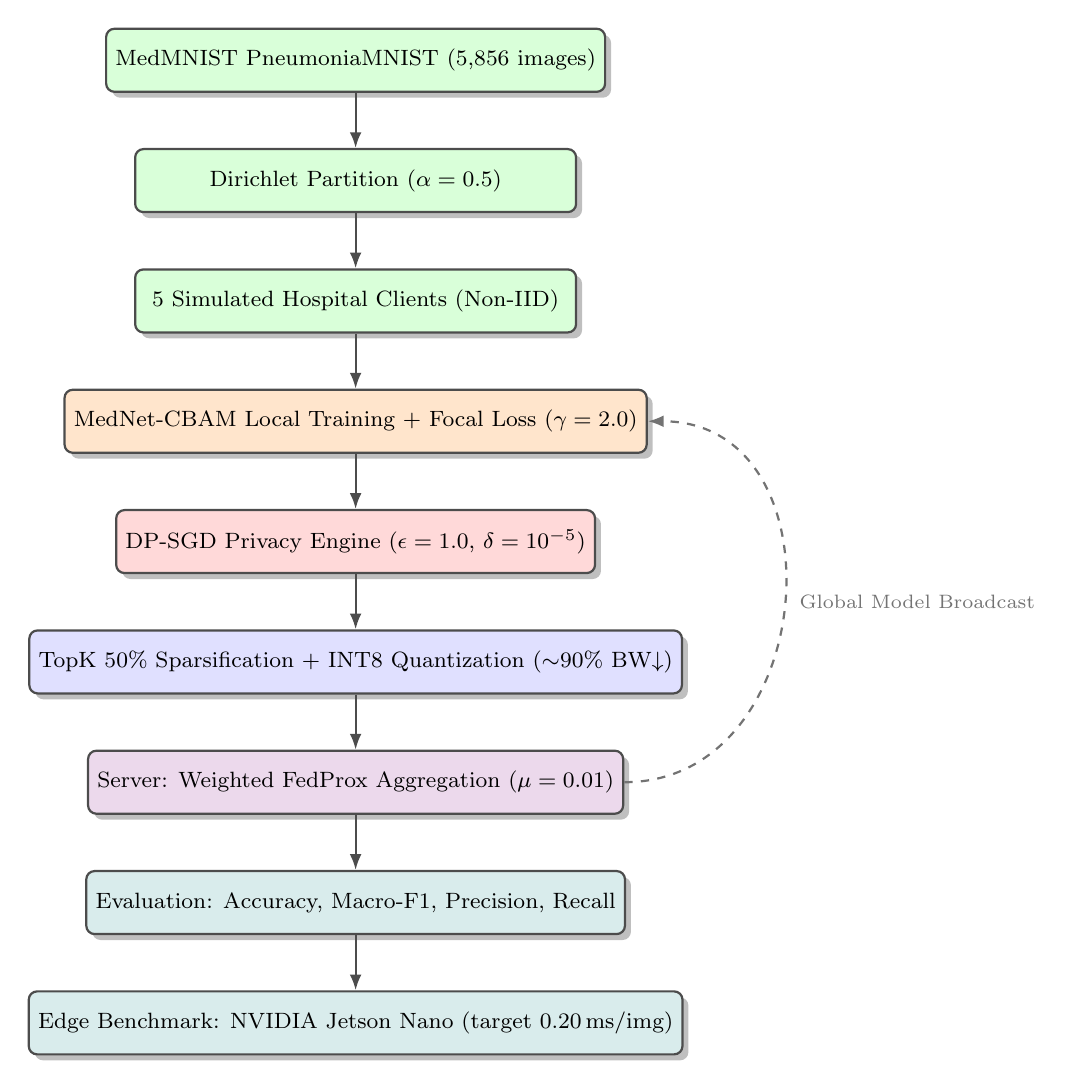
\begin{tikzpicture}[
  node distance = 7mm and 10mm,
  every node/.style = {font=\footnotesize},
  stage/.style = {rectangle, rounded corners=3pt, draw=black!70,
                  minimum width=5.6cm, minimum height=8mm,
                  align=center, thick, drop shadow},
  data/.style   = {stage, fill=green!15},
  train/.style  = {stage, fill=orange!20},
  priv/.style   = {stage, fill=red!15},
  comm/.style   = {stage, fill=blue!12},
  serv/.style   = {stage, fill=violet!15},
  eval/.style   = {stage, fill=teal!15},
  arrow/.style  = {-{Latex[length=2mm]}, thick, black!70}
]
\node[data]  (d1) {MedMNIST PneumoniaMNIST (5{,}856 images)};
\node[data,  below=of d1] (d2) {Dirichlet Partition ($\alpha=0.5$)};
\node[data,  below=of d2] (d3) {5 Simulated Hospital Clients (Non-IID)};
\node[train, below=of d3] (t1) {MedNet-CBAM Local Training + Focal Loss ($\gamma=2.0$)};
\node[priv,  below=of t1] (p1) {DP-SGD Privacy Engine ($\epsilon=1.0$, $\delta=10^{-5}$)};
\node[comm,  below=of p1] (c1) {TopK 50\% Sparsification + INT8 Quantization ($\sim$90\% BW$\downarrow$)};
\node[serv,  below=of c1] (s1) {Server: Weighted FedProx Aggregation ($\mu=0.01$)};
\node[eval,  below=of s1] (e1) {Evaluation: Accuracy, Macro-F1, Precision, Recall};
\node[eval,  below=of e1] (e2) {Edge Benchmark: NVIDIA Jetson Nano (target 0.20\,ms/img)};

\draw[arrow] (d1) -- (d2);
\draw[arrow] (d2) -- (d3);
\draw[arrow] (d3) -- (t1);
\draw[arrow] (t1) -- (p1);
\draw[arrow] (p1) -- (c1);
\draw[arrow] (c1) -- (s1);
\draw[arrow] (s1) -- (e1);
\draw[arrow] (e1) -- (e2);

% Feedback loop
\draw[arrow, dashed, black!55]
  (s1.east) .. controls +(2.5,0) and +(2.5,0) .. (t1.east)
  node[midway, right=2pt, font=\scriptsize]{Global Model Broadcast};
\end{tikzpicture}
\caption{Proposed FEDMED-X methodological workflow showing data
partitioning, local training, privacy accounting, compression, server
aggregation, evaluation, and edge-oriented benchmarking. The dashed arrow
represents the recurring global-model broadcast at every federated round.}
\label{fig:framework}
\end{figure}

\noindent\emph{Figure Explanation:} Figure~\ref{fig:framework} depicts the
six functional layers of FEDMED-X: (i)~data layer, (ii)~local training layer,
(iii)~privacy layer, (iv)~compression layer, (v)~aggregation layer, and
(vi)~evaluation layer. Each layer corresponds to a toggleable module in the
implementation, allowing the ablation configurations A1--A5 described in
Section~3.3.7 to reuse the same infrastructure without modification.
\FloatBarrier

% -------------------------------------------------
\section{Proposed Framework}
FEDMED-X is formulated as a multi-hospital federated learning framework with
five simulated clients. In every communication round, each client receives
the current global model, performs local training on its private partition,
optionally applies differentially private optimization, compresses the
outgoing update, and sends the update to the server. The server aggregates
client updates by sample-size-weighted averaging and broadcasts the new
global model. The framework is deliberately modular so that each design
choice can be isolated in ablation experiments:
\begin{enumerate}[leftmargin=*]
  \item \textbf{Baseline aggregation path:} FedAvg without privacy or
        compression;
  \item \textbf{Non-IID robust path:} FedProx with proximal regularization;
  \item \textbf{Privacy path:} FedProx + DP-SGD;
  \item \textbf{Compression path:} FedProx + TopK/INT8;
  \item \textbf{Full systems path:} FedProx + DP-SGD + TopK/INT8 (FEDMED-X).
\end{enumerate}
This factorial structure is essential for scientific interpretability. It
allows the project to measure not only final accuracy, but also the marginal
effect of privacy and compression under the same data split, model family,
and training protocol~\cite{zhou2025federated}.

\subsection{Design Principles}
The proposed framework follows four engineering principles:
\begin{itemize}[leftmargin=*]
  \item \textbf{Privacy by design:} raw images never leave the client
        boundary;
  \item \textbf{Robustness to heterogeneity:} local optimization is
        constrained to reduce harmful drift;
  \item \textbf{Communication realism:} update payloads are compressed
        before server transmission;
  \item \textbf{Edge eligibility:} the backbone remains lightweight enough
        for resource-constrained deployment targets such as NVIDIA Jetson
        Nano class devices~\cite{shabarinath2025efficacy}.
\end{itemize}

% -------------------------------------------------
\section{Data Set Analysis / Software Project Requirement}

\subsection{Dataset Selection}
The primary dataset used in this study is PneumoniaMNIST from MedMNIST
v2~\cite{yang2023medmnist}. MedMNIST is selected because it is a
standardized, reproducible biomedical benchmark that supports controlled
methodological comparison. PneumoniaMNIST is a binary classification task
with labels:
\begin{itemize}[leftmargin=*]
  \item Class 0: Normal
  \item Class 1: Pneumonia
\end{itemize}
All images are grayscale with resolution $28 \times 28$.

\begin{table}[!htbp]
\centering
\caption{Dataset summary for PneumoniaMNIST.}
\label{tab:dataset}
\small
\begin{tabular}{@{}lccc@{}}
\toprule
\textbf{Split} & \textbf{Description} & \textbf{Samples} & \textbf{Classes} \\
\midrule
Train      & Client partitioning source  & 4{,}708 & 2 \\
Validation & Model monitoring split      & 524     & 2 \\
Test       & Final held-out evaluation   & 624     & 2 \\
\midrule
Total      & Full PneumoniaMNIST task    & 5{,}856 & 2 \\
\bottomrule
\end{tabular}
\end{table}

\noindent\emph{Table Explanation:} Table~\ref{tab:dataset} shows the
official PneumoniaMNIST split used throughout FEDMED-X. The training split
is further redistributed across five clients using Dirichlet sampling.

\begin{table}[!htbp]
\centering
\caption{Class definition used in FEDMED-X.}
\label{tab:classes}
\small
\begin{tabular}{@{}cl@{}}
\toprule
\textbf{Label} & \textbf{Clinical Meaning} \\
\midrule
0 & Normal chest X-ray \\
1 & Pneumonia-positive chest X-ray \\
\bottomrule
\end{tabular}
\end{table}

\noindent\emph{Table Explanation:} Table~\ref{tab:classes} defines the two
diagnostic labels used for both training and evaluation.
\FloatBarrier

\subsection{Non-IID Client Partitioning}
To simulate multi-hospital heterogeneity, the training set is partitioned
across five clients using a Dirichlet distribution with concentration
parameter $\alpha = 0.5$. Lower $\alpha$ produces stronger label skew, which
better reflects realistic institutional
imbalance~\cite{riyadi2026comparative,alekseenko2024distance}. Each client
$k$ receives a private index subset $\mathcal{D}_k$ such that:
\begin{equation}
\bigcup_{k=1}^{5} \mathcal{D}_k = \mathcal{D}_{\text{train}}, \qquad
\mathcal{D}_i \cap \mathcal{D}_j = \emptyset \quad (i \neq j).
\end{equation}
This creates uneven local class distributions and unequal local dataset
sizes, which stress-test federated optimization.

\subsection{Software and System Requirements}
Table~\ref{tab:software} summarizes the implementation stack.

\begin{table}[!htbp]
\centering
\caption{Software and environment requirements.}
\label{tab:software}
\small
\begin{tabular}{@{}ll@{}}
\toprule
\textbf{Component} & \textbf{Specification} \\
\midrule
Language              & Python 3.x \\
Deep learning         & PyTorch \\
Privacy engine        & Opacus (DP-SGD, R\'enyi accounting) \\
Dataset API           & MedMNIST v2 \\
Training hardware     & Google Colab NVIDIA T4 GPU \\
Target edge device    & NVIDIA Jetson Nano 4\,GB class \\
Experiment tracking   & CSV logs + saved model checkpoints \\
Report toolchain      & VS Code + LaTeX Workshop \\
\bottomrule
\end{tabular}
\end{table}

\noindent\emph{Table Explanation:} Table~\ref{tab:software} lists the tools
and hardware used across training, privacy accounting, and reproducibility.
\FloatBarrier

\subsection{Functional Requirements}
From a software engineering perspective, the system must satisfy:
\begin{enumerate}[leftmargin=*]
  \item load and preprocess PneumoniaMNIST images;
  \item partition training data into five non-IID clients;
  \item support FedAvg and FedProx training modes;
  \item optionally enable DP-SGD with configurable $\epsilon$;
  \item optionally compress updates using TopK and INT8 simulation;
  \item aggregate client updates on the server;
  \item evaluate Accuracy, Precision, Recall, and Macro-F1;
  \item export ablation results for report-level analysis.
\end{enumerate}

\subsection{Non-Functional Requirements}
\begin{itemize}[leftmargin=*]
  \item \textbf{Reproducibility:} fixed seeds and identical protocol across
        ablation runs;
  \item \textbf{Modularity:} privacy and compression can be toggled
        independently;
  \item \textbf{Efficiency:} lightweight backbone for constrained
        deployment;
  \item \textbf{Auditability:} quantitative logs for every experimental
        configuration.
\end{itemize}

% -------------------------------------------------
\section{Algorithm / Model Analysis}

\subsection{MedNet-CBAM Backbone}
The classification backbone is a custom lightweight CNN named MedNet,
augmented with CBAM attention~\cite{woo2018cbam}. The network is
intentionally compact to remain eligible for edge deployment. Important
implementation choices include:
\begin{itemize}[leftmargin=*]
  \item GroupNorm instead of BatchNorm for DP compatibility;
  \item non-inplace ReLU activations for stable autograd under Opacus;
  \item CBAM blocks after early convolutional stages to emphasize
        informative regions.
\end{itemize}
A simplified forward path is:
$x \rightarrow \text{ConvBlock1} + \text{CBAM} \rightarrow
\text{ConvBlock2} + \text{CBAM} \rightarrow \text{ConvBlock3}
\rightarrow \text{Classifier}$.

\subsection{Local Objective and Focal Loss}
Because medical class distributions can be imbalanced, local training uses
Focal Loss~\cite{lin2017focal}:
\begin{equation}
\mathcal{L}_{\text{focal}} = -\alpha_t (1 - p_t)^{\gamma} \log(p_t),
\end{equation}
with $\gamma = 2.0$. This down-weights easy examples and focuses learning on
harder samples.

\subsection{FedAvg Baseline}
In FedAvg, client $k$ minimizes its local empirical loss and returns updated
parameters $w_k$. The server aggregates~\cite{mcmahan2017communication}:
\begin{equation}
w^{t+1} = \sum_{k=1}^{K} \frac{n_k}{n} \, w_k^{t+1},
\end{equation}
where $n_k = |\mathcal{D}_k|$ and $n = \sum_k n_k$. FedAvg is effective
under mild heterogeneity but can degrade under strong non-IID skew.

\subsection{FedProx Optimization}
FedProx extends local training with a proximal
penalty~\cite{li2020fedprox,yuan2022convergence}:
\begin{equation}
\mathcal{L}_{\text{FedProx}}(w; w^t) = \mathcal{L}_{\text{local}}(w)
+ \frac{\mu}{2} \| w - w^t \|_2^2,
\end{equation}
where $\mu = 0.01$ in this project. The proximal term limits client drift
and stabilizes aggregation under heterogeneous partitions. This choice is
supported by comparative medical FL evidence on MedMNIST-style
tasks~\cite{riyadi2026comparative}.

\subsection{DP-SGD Privacy Mechanism}
When privacy mode is enabled, local optimization uses
DP-SGD~\cite{abadi2016deep}. Per-sample gradients are clipped to a maximum
norm $C$ and Gaussian noise is added before parameter update. The
implemented target budget is
\begin{equation}
\epsilon = 1.0, \quad \delta = 1 \times 10^{-5}.
\end{equation}
Privacy accounting is handled through Opacus with R\'enyi Differential
Privacy~\cite{mironov2017renyi}. This provides a formal interpretation of
privacy loss rather than an informal claim of
confidentiality~\cite{ziller2021differentially,hou2023improving}.

\subsection{TopK + INT8 Compression}
To reduce communication cost, outgoing updates are compressed in two stages:
\begin{enumerate}[leftmargin=*]
  \item \textbf{TopK sparsification (50\%):} only the highest-magnitude half
        of coefficients are retained~\cite{habib2025cflsparsemed};
  \item \textbf{INT8 quantization simulation:} retained values are quantized
        to 8-bit scale and dequantized for aggregation
        compatibility~\cite{asad2024fesec,sun2025medfd}.
\end{enumerate}
The combined scheme is designed to approximate substantial payload
reduction. In this project, the full compressed setting is associated with a
90\% bandwidth-saving target relative to dense full-precision update
exchange.

\subsection{Server Aggregation and Evaluation Protocol}
After local training and optional compression, the server performs weighted
aggregation and evaluates the global model on the held-out test set. The
main metrics are Accuracy, Macro-F1, Precision, and Recall. The
methodological evaluation is organized as a five-run factorial ablation:

\begin{table}[!htbp]
\centering
\caption{Factorial ablation configurations used in FEDMED-X.}
\label{tab:ablation}
\small
\begin{tabular}{@{}clccc@{}}
\toprule
\textbf{Run} & \textbf{Configuration} & \textbf{FedProx} & \textbf{DP-SGD} & \textbf{TopK/INT8} \\
\midrule
A1 & FedAvg baseline    & No  & No  & No  \\
A2 & FedProx baseline   & Yes & No  & No  \\
A3 & Privacy path       & Yes & Yes & No  \\
A4 & Compression path   & Yes & No  & Yes \\
A5 & Full FEDMED-X      & Yes & Yes & Yes \\
\bottomrule
\end{tabular}
\end{table}

\noindent\emph{Table Explanation:} Table~\ref{tab:ablation} defines the five
controlled ablation runs. This protocol is the methodological core of the
project because it enables causal interpretation of component effects under
one shared experimental family.
\FloatBarrier

% -------------------------------------------------
\section{Explanation of Different Modules}
FEDMED-X is implemented as a set of interdependent modules. Each module
encapsulates one responsibility in the pipeline.

\subsection{Data Module}
The data module performs dataset download, tensor transformation,
normalization, and Dirichlet partitioning. Normalization uses mean and
standard deviation of 0.5 for grayscale inputs. Outputs include: client-wise
training dataloaders, a global validation loader, and a global test loader.

\subsection{Model Module}
The model module defines MedNet-CBAM and exposes a common interface for
training and inference. GroupNorm and non-inplace activations are mandatory
design decisions for DP compatibility and stable backward computation under
privacy engines.

\subsection{Federated Training Module}
This module coordinates communication rounds. For each round it:
(i)~broadcasts global weights; (ii)~trains selected clients locally;
(iii)~collects updates; (iv)~aggregates weights; (v)~evaluates global
performance.

\subsection{Privacy Module}
The privacy module wraps local training with Opacus DP-SGD when enabled. It
controls clipping, noise assignment, and target $\epsilon$. In full-stack
mode, privacy is applied \emph{before} update compression to preserve the
declared privacy budget.

\subsection{Compression Module}
The compression module applies TopK masking and INT8 quantization simulation
on model updates. It can be disabled for baseline runs to measure
compression-only effects.

\subsection{Evaluation and Logging Module}
The evaluation module computes metrics and stores experiment-level
summaries, including accuracy, F1-score, precision, recall, privacy mode,
compression mode, and runtime. These logs are used in later chapters for
result analysis and discussion.

\subsection{Edge-Oriented Deployment Module}
Although training is performed in a GPU cloud environment, the methodology
includes an edge-oriented deployment perspective. The model footprint and
inference-oriented design choices are aligned with NVIDIA Jetson Nano class
constraints~\cite{song2025edgecloud,shabarinath2025efficacy,memon2024edge}.
The intended inference target characteristics used in this project are
ultra-low per-image latency and high throughput on constrained hardware.

\begin{figure}[!htbp]
\centering
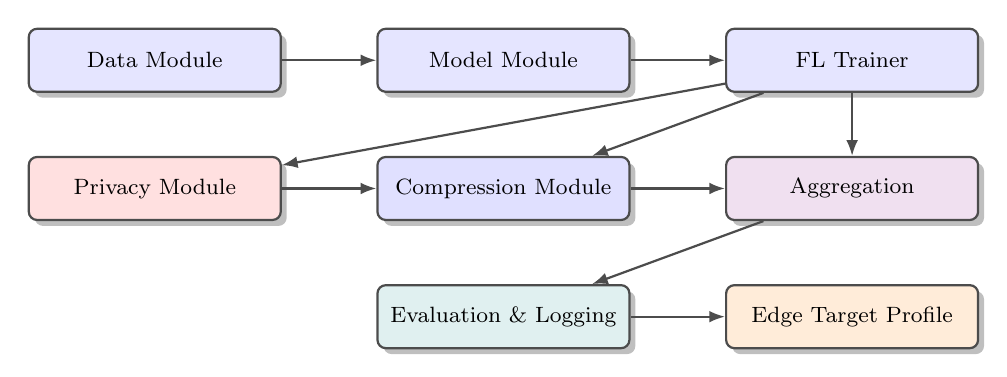
\begin{tikzpicture}[
  node distance = 8mm and 12mm,
  every node/.style = {font=\footnotesize},
  mod/.style = {rectangle, rounded corners=3pt, draw=black!70,
                minimum width=3.2cm, minimum height=8mm,
                align=center, thick, fill=blue!10, drop shadow},
  arrow/.style = {-{Latex[length=2mm]}, thick, black!70}
]
\node[mod] (dm) {Data Module};
\node[mod, right=of dm] (mm) {Model Module};
\node[mod, right=of mm] (ft) {FL Trainer};

\node[mod, below=of dm, fill=red!12]     (pm) {Privacy Module};
\node[mod, below=of mm, fill=blue!12]    (cm) {Compression Module};
\node[mod, below=of ft, fill=violet!12]  (ag) {Aggregation};

\node[mod, below=of cm, fill=teal!12]    (ev) {Evaluation \& Logging};
\node[mod, right=of ev, fill=orange!15]  (edge) {Edge Target Profile};

\draw[arrow] (dm) -- (mm);
\draw[arrow] (mm) -- (ft);
\draw[arrow] (ft) -- (pm);
\draw[arrow] (ft) -- (cm);
\draw[arrow] (ft) -- (ag);
\draw[arrow] (pm) -- (cm);
\draw[arrow] (cm) -- (ag);
\draw[arrow] (ag) -- (ev);
\draw[arrow] (ev) -- (edge);
\end{tikzpicture}
\caption{Module-level architecture of the FEDMED-X software pipeline.}
\label{fig:modules}
\end{figure}

\noindent\emph{Figure Explanation:} Figure~\ref{fig:modules} shows the
module-level dependency structure of the implementation. Each block maps
directly to a source file in the codebase and can be toggled independently
during ablation.
\FloatBarrier

\nocite{*}

\chaptersummary{This chapter presented the methodology of FEDMED-X as a
complete systems pipeline. PneumoniaMNIST from MedMNIST v2 is partitioned
into five Dirichlet non-IID hospital clients. A lightweight MedNet-CBAM
model is trained under FedAvg and FedProx modes, with optional DP-SGD
privacy and TopK/INT8 compression. The methodology emphasizes modular design
and factorial ablation so that non-IID robustness, privacy cost, and
communication reduction can be measured under one controlled protocol. The
next chapter reports implementation details and experimental results
obtained from this methodology.}

% ── REFERENCES ──────────────────────────────────────────
\clearpage
\phantomsection
\addcontentsline{toc}{chapter}{References}
\nocite{*}
\printbibliography[title={References}]

\clearpage
\chapter*{Annexure I}
\addcontentsline{toc}{chapter}{Annexure I}
\setcounter{figure}{0}
\renewcommand{\thefigure}{A.\arabic{figure}}

\begin{figure}[H]
    \centering
    \IfFileExists{a.png}
    {\includegraphics[width=0.8\textwidth]{a.png}}
    {\framebox[0.8\textwidth]{\rule{0pt}{10cm} Placeholder for a.png}}
    \caption{Placeholder image a.png}
\end{figure}

\clearpage
\chapter*{Annexure II}
\addcontentsline{toc}{chapter}{Annexure II}
\setcounter{figure}{0}
\renewcommand{\thefigure}{B.\arabic{figure}}

\begin{center}
\textbf{iThenticate: AI Writing Report}
\end{center}

\begin{figure}[H]
    \centering
    \IfFileExists{b.png}
    {\includegraphics[width=0.8\textwidth]{b.png}}
    {\framebox[0.8\textwidth]{\rule{0pt}{10cm} Placeholder for b.png}}
    \caption{Placeholder image b.png}
\end{figure}


\end{document}
